\chapter{実際にあった論文の不備ツアー}

% 本章では、過去に提出された卒業論文において実際にあった不備の例を示す。


% \section{不必要に大きな図}

% 内容とは関係の薄い小さな図を大幅に拡大して1ページを使っていた(\figref{fig:fail-root})。
% 同様の行為を2,3ページに渡って繰り返すことで規定のページ数に達するよう水増ししていた\footnote{内容と関係する重要な図・元々大きな図であれば,大きく掲載しても問題はありません}。


% \begin{figure}[H]
%   \centering
%   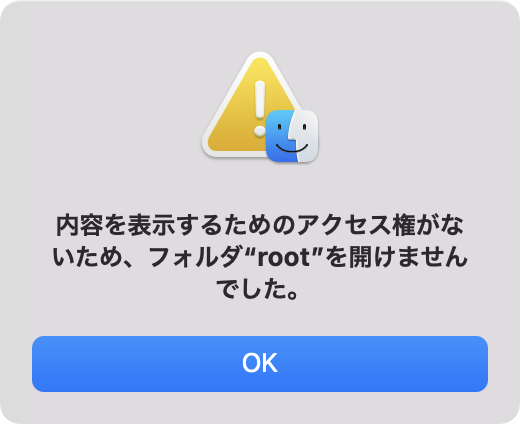
\includegraphics[width=.90\linewidth]{fig/fail-root.png}
%   \caption{不必要に大きな図によるページ稼ぎ}
%   \label{fig:fail-root}
% \end{figure}


% \section{テンプレートの修正漏れ}

% テンプレートに入っている仮の研究室名が修正されていなかった(\figref{fig:fail-cover})。
% 10年以上前には提出者の氏名が「工科太郎」のままの人もいた。
% 先輩の論文をテンプレートにしたのか、年度・日付がすべて前年度のものになっている論文もあった。

% \begin{figure}[H]
%     \centering
%     \fbox{
%         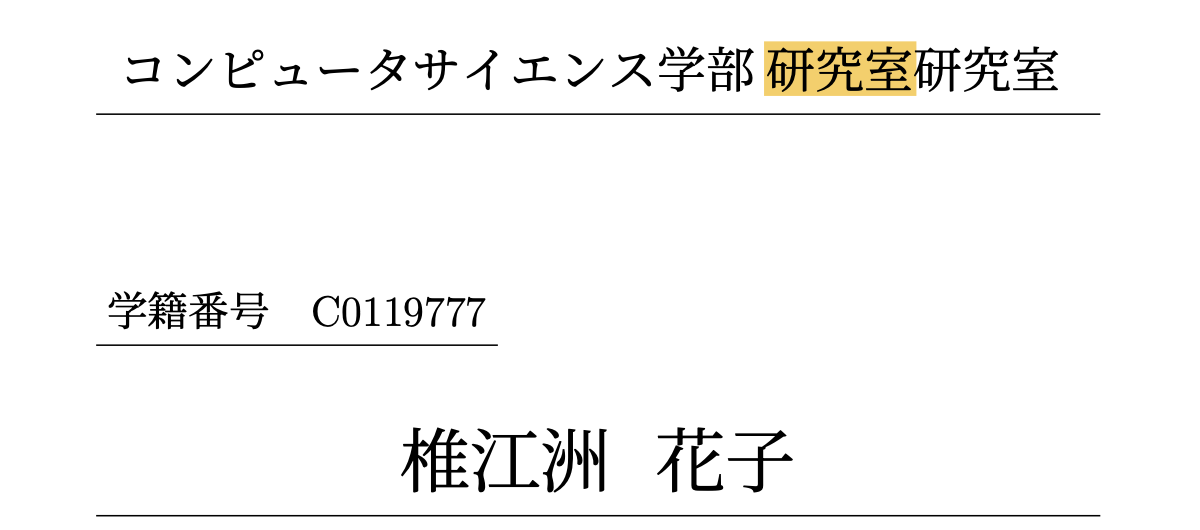
\includegraphics[width=.5\linewidth]{fig/fail-cover2.png}
%     }
%     \caption{テンプレートの修正漏れ}
%     \label{fig:fail-cover}
% \end{figure}

% \section{年度・年・日付}

% 提出日の「年」を間違えてしまった。
% 表紙には「年度」を記入する(\figref{fig:fail-year01})。
% 内表紙には「提出年月日」を記入する(\figref{fig:fail-year02})。
% 概要には「年度」を記入する(\figref{fig:fail-year03})。
% 後期(1月)に卒業論文を提出する場合、年度と提出年は異なる。
% 前期(7月)に卒業論文を提出する場合、年度と提出年は等しい。

% \begin{figure}[htbp]
%   \begin{minipage}[b]{0.5\linewidth}
%     \centering
%     \fbox{
%       
\includegraphics[scale=.5]{fig/fail-year01.png}
%     }
%     \caption{表紙(年度)}
%     \label{fig:fail-year01}
%   \end{minipage}
%   \begin{minipage}[b]{0.5\linewidth}
%     \centering
%     \fbox{
%       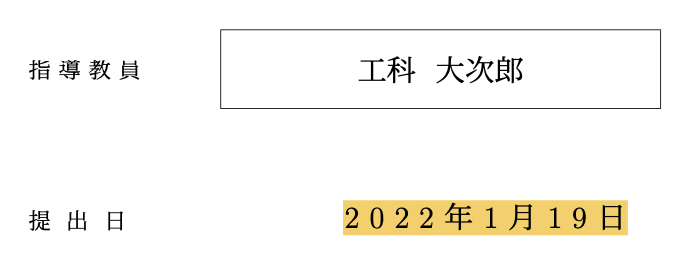
\includegraphics[scale=.5]{fig/fail-year02.png}
%     }
%     \caption{内表紙(年)}
%     \label{fig:fail-year02}
%   \end{minipage}
% \end{figure}

% \begin{figure}
%     \centering
%     \fbox{
%       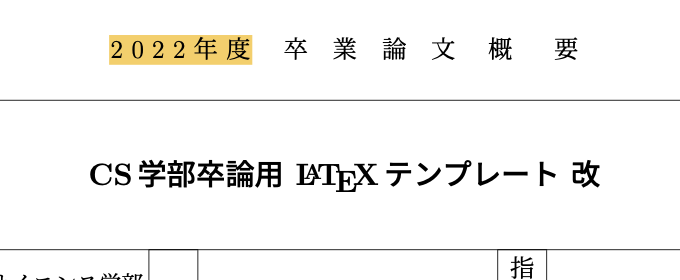
\includegraphics[scale=.8]{fig/fail-year03.png}
%     }
%     \caption{概要(年度)}
%     \label{fig:fail-year03}
% \end{figure}


% \section{フォント}

% 途中からフォントサイズが不自然に大きくなった(\figref{fig:fail-font})。

% \begin{figure}[H]
%     \centering
%     \fbox{
%         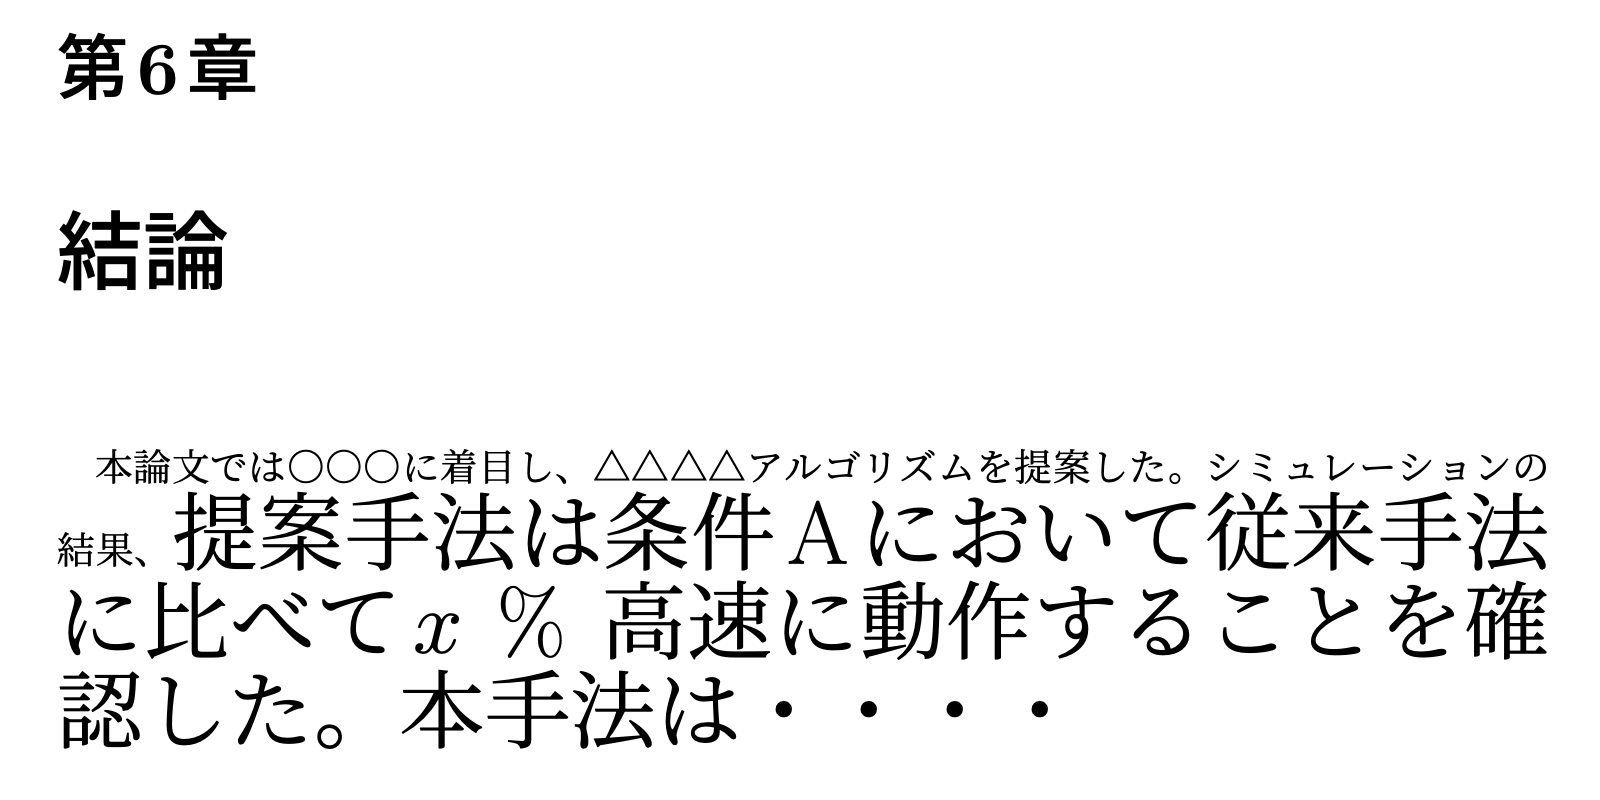
\includegraphics[width=.45\linewidth]{fig/fail-font.png}
%     }
%     \caption{フォントサイズ変更によるページ稼ぎ}
%     \label{fig:fail-font}
% \end{figure}


% \section{学籍番号}

% 先頭のCを小文字にしてしまった(\figref{fig:fail-id})。
% 学籍番号のC(学部)、A(先進情報)、B(人工知能)は大文字を使うこと。

% \begin{figure}[H]
%     \centering
%     \fbox{
%         
\includegraphics[width=.45\linewidth]{fig/fail-id.png}
%     }
%     \caption{学籍番号の間違い}
%     \label{fig:fail-id}
% \end{figure}

% \setcounter{section}{6}
% \section{章立て}

% 章・節・項の番号が連続していなかった(例:この節および次の節)。

% \setcounter{section}{6}
% \section{図表}

% 図の番号が「章番号 . 図番号」の形式ではなかった。
% \figref{fig:fail-fig}は論文の最初から数えれば11番目の図であるが、5章の中では8番目の図である。

% \begin{figure}[H]
%   \centering
%   \fbox{
%       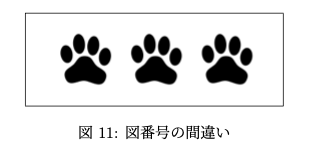
\includegraphics[width=.5\linewidth]{fig/fail-fig.png}
%   }
%   \caption{図番号の間違い}
%   \label{fig:fail-fig}
% \end{figure}

% 表のキャプションが下にあるケースも多かった(\tabref{tab:noffaculties})。
% 表のキャプションは表の上につけよう。

% \begin{table}[htbp]
% 	\centering
% 	\begin{tabular}{l|r}
% 		\hline \hline
% 		所属 & 人数 (人)\\
% 		\hline
% 		八王子 & 152\\
%     蒲田 & 117\\
%     教養学館 & 18\\
%     片柳研究所 & 7\\
%     センター関係 & 4\\
% 		\hline
% 	\end{tabular}
%   \caption{東京工科大学の教員数(所属別)}
%   \label{tab:noffaculties}
% \end{table}

% %%%%%%%%%%%%%%%%%%%%%%%%%%%%%%%%%%%%%%%%%%%%%%%%%%%%%%%%%%%%%%%%%%%%%%%
% \begin{comment}
%   \begin{textblock}{5}(14, 8.5)
%     \noindent
%     表のキャプションは表の上
%   \end{textblock}
  
%   \begin{textblock}{3}(16, 16)
%     \noindent
%     ←2.2節がない
%   \end{textblock}
% \end{comment}
% %%%%%%%%%%%%%%%%%%%%%%%%%%%%%%%%%%%%%%%%%%%%%%%%%%%%%%%%%%%%%%%%%%%%%%%


% \section{目次}

% 論文の章立てと目次とが一致しなかった(\figref{fig:fail-index})。

% \begin{figure}[H]
%   \centering
%   \fbox{
%     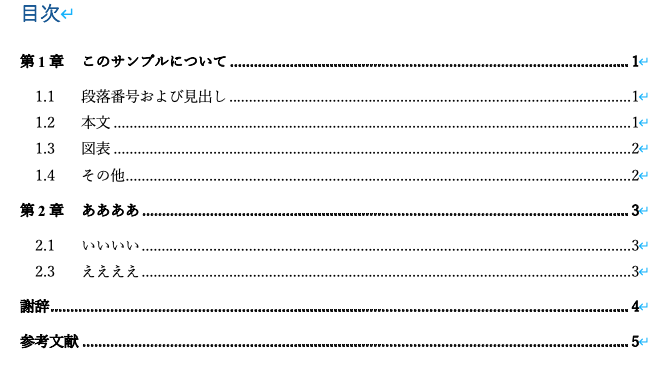
\includegraphics[width=.65\linewidth]{fig/fail-index.png}
%   }
%   \caption{目次の間違い}
%   \label{fig:fail-index}
% \end{figure}

% \section{謝辞}

% 謝辞が祝辞だった(\figref{fig:fail-ack})。信じられないかもしれないけれど、本当にあった(確か2005年度)。

% \begin{figure}[H]
%     \centering
%     \fbox{
%         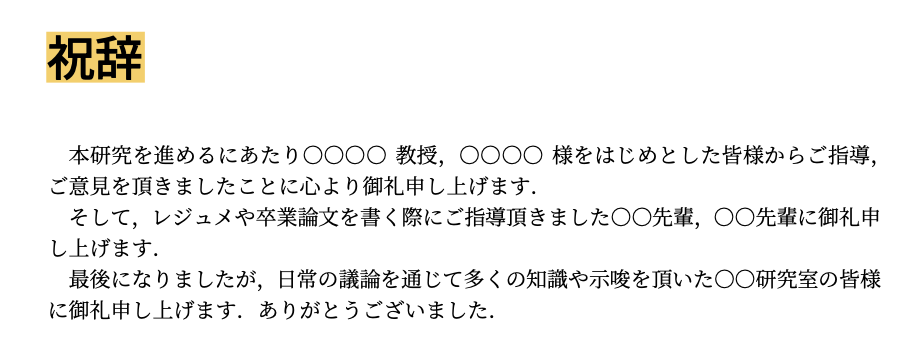
\includegraphics[width=.6\linewidth]{fig/fail-ack.png}
%     }
%     \caption{祝いの言葉}
%     \label{fig:fail-ack}
% \end{figure}